\section{ELKStack}
\label{chapter:application:elkstack}

\textbf{ELKStack} - akronim opisujący stos technologi składający się z 3 elementów:
\begin{itemize}
    \item[ElasticSearch] - pełnotekstowy silnik wyszukiwania,
    \item[Logstash] - scentralizowane przetwarzania danych,
    \item[Kibana] - interfejs graficzny silnika \textbf{ElasticSearch}
\end{itemize}

\subsection{Logstash}
    Logstash jest wysoce elastycznym narzędziem, nie tylko w kontekście architektury \textbf{ELKStack}.
    Możliwe jest skonfigurowanie go, aby działał jako kolektor danych, jako ich filtr czy też
    transformator. Składa się on z 3 elementów:
    \begin{itemize}
        \item sekcji wejścia,
        \item sekcji przetwarzania,
        \item sekcji wyjścia
    \end{itemize}
    Każda z nich może składać się z więcej niż jednego bloku, opisującego jej zadania.
    Innymi słowy ilość wejść jest nieograniczona tak samo jak możliwości przetworzenia
    odebranych danych oraz ostatecznie wysłania ich do więcej niż jednej lokalizacji.
    Ponadto dla każdej z nich możliwe jest napisania własnego modułu lub wykorzystanie
    jednego z, ciągle rosnącej listy, publicznie dostępnych.
    
    Jest to ponadto rozwiązanie szybkie oraz łatwo skalowalne. Uruchomienie kolejnej
    instancji sprowadza się do przygotowania odpowiedniego pliku konfiguracyjnego
    i dostarczenia go jako argumentu wejściowego do pliku wykonywalnego aplikacji Logstash.
    Dzięki ciągle rozbudowywanej bazie wtyczek potrafi on jednak o wiele więcej. 
    Rozszerzenia można podzielić na 3 grupy, które odpowiadają omówionych wyżej sekcjom.
    Możliwe jest wybranie dowolnego rodzaju źródła danych. Nie musi być nim wcale plik fizyczny.
    Logstash może czytać także z kolejek, takich jak Kafka, bazy danych lub socket'ów.
    W sekcji przetwarzania można umieścić logikę odpowiedzialną za dodawania, usuwania poszczególnych
    pól. Możliwe jest także umieszczenie w środku małego programu napisanego w języku Ruby, jeśli
    jest to konieczne. Ostatecznie, ilość obsługiwanych wyjść można zacząć opisywać od innego
    elementu stosu technologicznego jakim jest \textbf{ELKStack}, czyli samej bazy danych
    \textbf{ElasticSearch}, a zakończyć na wypisywaniu kolejnych wydarzeń na konsolę. 

\subsection{ElasticSearch}
\label{chapter:application:elkstack:elasticsearch}
    Pełnotekstowych, indeksowany silnik wyszukiwania. Jednak \textbf{ElasticSearch} jest także
    nierelacyjną bazą danych opartą o koncepcję dokumentów. Możliwość przechowywania oraz wyszukiwania
    informacji pośród zgromadzonych danych, które mogą mieć zarówno ustaloną strukturę, jak i  luźną, jest
    szczególnie istotna dla zarządzania logami. Tym co wyróżnia każdy z nich jest informacja, wiadomość
    zawarta w kolejnych rekordach, a która jest inna dla każdego z nich. 
    
    ElasticSearch oferuje możliwość pełnotekstowej wyszukiwarki na przechowywanych danych, dzięki
    indeksacji. Każda informacja, która wpływa do aplikacji, nie jest po prostu tam zapisywana.
    Specjalnie skonfigurowane indeksy pozwalają na określenie tego, co jest istotne. Ale nie jest
    to konieczne. Jedną z wartych wspomnienia funkcji, jest automatyczna detekcja typów danych, na ich
    podstawie. Wspomniane indeksy są tworzone automatycznie, aby jak najszybciej można było
    wykorzystać możliwości oferowane przez \textbf{ElasticSearch}.
    
    \textbf{Multitenancy}, cecha, wyróżnik chmur obliczeniowych, jest bardzo łatwo do osiągnięcia
    dzięki grupowania i indeksacji w \textbf{ElasticSearch}. Grupa idealnie oddaje koncepcję tenanta.
    Wszystkie dane dla niego zgromadzone mogą zostać odszukane, poprzez wskazania indeksu. Jest on
    tożsamy z grupą, a w dalszej kolejności tenantem.
    
    Jest to także rozwiązania łatwo skalowalne. \textbf{ElasticSearch} posiada ten mechanizm wbudowany.
    Innymi słowy każda nowo uruchomiana instancja poszukuje w sieci, w której działa, innych instancji
    samoistnie budując klaster złożony z lidera oraz replik. 
    Lider odpowiedzialny jest za koordynacją pracy klastra i może również przechowywać dane.
    Repliki stanowią odzwierciedlenie stanu lidera. Jeśli którakolwiek z instancji zostanie wyłączona z klastra,
    potrafi się o samodzielnie przebudować. Dane przesyłane są między replikami. Ostatecznie uzyskuje się
    stan równowagi. Utracenie lidera nie stanowi przeszkody dla poprawnego działania. Pozostałe maszyny 
    negocjują wybór nowego i całość jest ponownie gotowa do świadczenia pełnej funkcjonalności w relatywnie
    krótkim czasie.
    
    \begin{figure}[h]
        \centering
        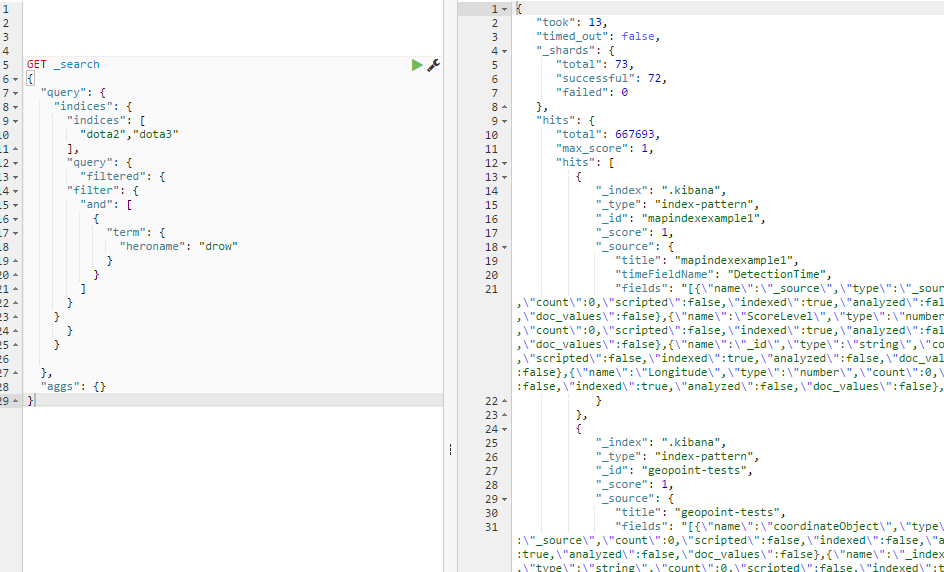
\includegraphics[width=1.0\textwidth]{images/es_query}
        \caption[Przykładowe zapytania do ElasticSearch]{
            Przykładowe zapytania do ElasticSearch, źródło: \url{http://i.stack.imgur.com/GFMUd.png}
        }
        \label{chapter:application:elkstack:es:query}
    \end{figure}

    Ostatecznie jest to także \textbf{REST}-owe API. Cała funkcjonalność dostępne jest poprzez
    protokół HTTP. Możliwe jest również administrowaniem klastra przez to samo medium.

\clearpage    
\subsection{Kibana}
\label{chapter:application:elkstack:kibana}

    Ostatni z elementów \textbf{ELKStack}. Zadaniem \textbf{Kibana} jest dostarczyć graficznego interfejsu
    użytkownika dla \textbf{ElasticSearch}. Z poziomu aplikacji dostępnej przez przeglądarkę możliwe
    jest przeglądania wszystkich danych zgromadzonych przez \textbf{Logstash} z użyciem tradycyjnych
    metod przeszukiwania:
    \begin{itemize}
        \item filtrowanie,
        \item kwerendy, w tym wypadku pełnotekstowe
    \end{itemize}
    
    Niemniej, to co jest szczególnie użyteczne to wizualizacja danych. Domyślny widok pozwala przeglądać 
    rekordy w formie zbliżonej do tabeli. 
    \begin{figure}[h]
        \centering
        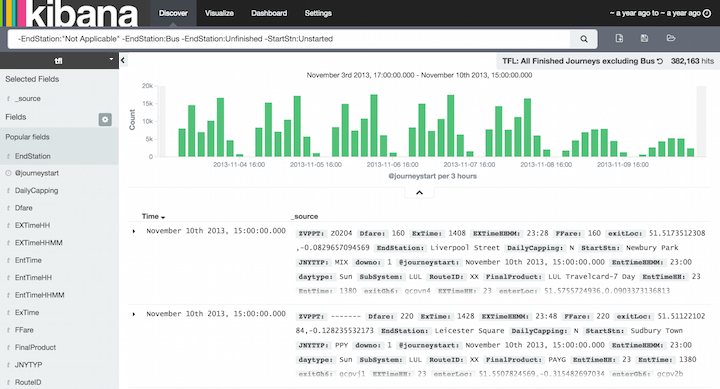
\includegraphics[width=1.0\textwidth]{images/kibana_main_view}
        \caption[Ekran główny w Kibana]{
            Ekran główny w Kibana, źródło: \url{https://www.elastic.co/guide/en/kibana/current/introduction.html}
        }
        \label{chapter:application:elkstack:kibana:main_view}
    \end{figure}
    W tym samym miejscu, można zaobserwować jak Kibana współpracuje z ElasticSearch. Na rysunku \ref{chapter:application:elkstack:kibana:main_view} po lewej stronie widoczny jest pasek szybkiego
    wyszukiwania. Znajdujące się tam pozycje odpowiadają kolejnym właściwościom przeglądanego zbioru danych.
    Korzystając z niego, potencjalny użytkownik, ma możliwość szybkiego filtrowania danych, a ilość filtrów jest
    nieograniczona. Po włączeniu wszystkich szybkiej filtracji, użytkownik w dalszym ciągu, może napisać
    własne zapytania \textbf{QueryDSL} i przesłać je do serwera. Kibana, domyślnie, sortuje dane w kolejności
    rosnącej względem skonfigurowanego pola dla danego indeksu. Rekordy można oglądać w dowolnym wycinku czasu.
    
    Szczególnie interesującą cechą wyników wyszukiwań, które można przeglądać w Kibana, jest to, że bezboleśnie
    łączą się one z dowolną formą wizualizacji. I tak samo, jak użytkownik, mógłby chcieć przejrzeć dane 
    jedynie z konkretnych dwóch godzin, konkretnego dnia, tak samo, możliwe jest uruchomienie podobnego
    filtru dla wykresu kołowego lub słupkowego.
    \begin{figure}[H]
        \centering
        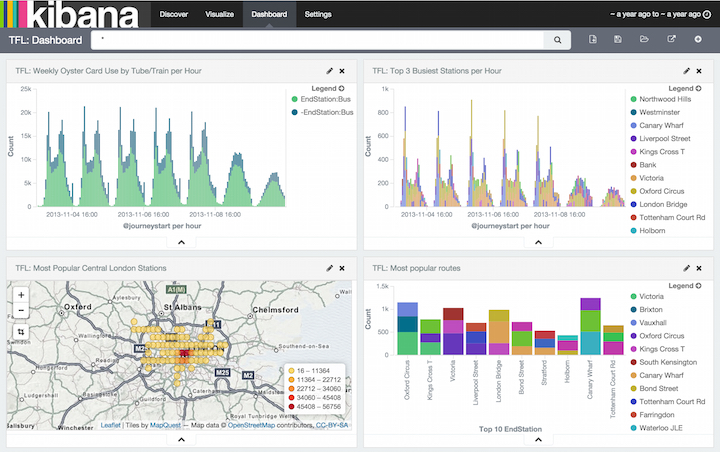
\includegraphics[width=1.0\textwidth]{images/kibana_dashboards}
        \caption[Ekran współdzielony w Kibana]{
            Ekran współdzielony w Kibana, źródło: \url{https://www.elastic.co/guide/en/kibana/current/introduction.html}
        }
        \label{chapter:application:elkstack:kibana:dashboard}
    \end{figure}
    Wykresy, w dalszym ciągu można łączyć w tak zwane \textbf{dashboards}, które stanowią idealne narzędzia do kolaboracji
    w tym samym zespole. Prócz tego, że pozwalają ona na pokazanie jednocześnie więcej niż jednej wizualizacji, z których
    każda odnosi się do samego momentu w czasie, da się je zapisywać i przekazywać innym członkom zespołu. 